\subsection{Logic gates}

\begin{definition}
	A \emph{transistor} is an electronic device that has three terminals:
	a \emph{source}, a \emph{drain}, and a \emph{gate}.
	The drain and source are connected depending on the voltage of the gate.
\end{definition}

The most common transistor is the
\emph{metal-oxide-semicoductor field-effect transistor} (MOSFET),
which can be \emph{n-type} (if the voltage of the gate is high, the drain
and source are connected) or \emph{p-type} (if the voltage of the gate is low,
the drain and source are connected).

\begin{figure}
    \centering
    \begin{circuitikz}
        \draw
            (0,0) node[nmos] (nmos) {}
            (nmos.base) node[left] {$g$}
            (nmos.collector) node[above] {$d$}
            (nmos.emitter) node[below] {$s$}
        ;
    \end{circuitikz}
    \hspace{4em}
    \begin{circuitikz}
        \draw
            (0,0) node[pmos] (pmos) {}
            (pmos.base) node[left] {$g$}
            (pmos.collector) node[below] {$d$}
            (pmos.emitter) node[above] {$s$}
        ;
    \end{circuitikz}
    \caption{Diagrams for a nMOS (left) and a pMOS (right) transistor where $d$ is the drain, $s$ is the source, and  $g$ is the gate.}
    \label{fig:nmos_pmos}
\end{figure}

\begin{definition}[Capacitor]
	A \emph{capacitor} is two pieces of conductive material separated by an
	insulator.
	If a positive voltage is applied to one side, it accumulates a charge
	$Q$ and the other side accumulates the opposite charge $-Q$.
	It takes time and energy to charge of discharge a capacitor.
\end{definition}

\begin{figure}
	\centering
	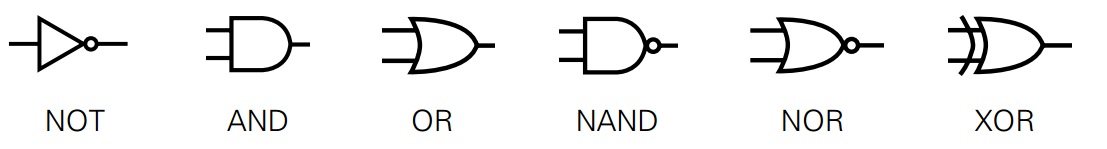
\includegraphics[width=\textwidth]{images/logic-gates}
	\caption{Logic gate diagrams.}
	\label{fig:logic-gates}
\end{figure}

Figure \ref{fig:logic-gates} shows the symbol for different types of
logic gates.

The following is the truth tables for XOR ($\oplus$).

\begin{center}
	\begin{tabular}{ccc}
		\toprule
		$A$ & $B$ & $A \oplus B$ \\
		\midrule
		0 & 0 & 1 \\
		0 & 1 & 0 \\
		1 & 0 & 0 \\
		1 & 1 & 0 \\
		\bottomrule
	\end{tabular}
\end{center}

Now we will move onto constructing logic gates from transistors. 
Figure \ref{fig:not-cmos-schematic} shows the schematic
of a NOT gate using CMOS transistors.
Similarly, Figure \ref{fig:nand-cmos-schematic} shows the schematic of a
NAND gate using CMOS transistors.

\begin{figure}
    \centering
    \begin{circuitikz}
    	\draw
    		(1,1) node[pmos] (pmos) {}
    		(1,-1) node[nmos] (nmos) {}
    		(-0.5,0) node[left] {$A$} -- (0,0)
    		(2,0) node[right] (S) {$S$}
    		(pmos.emitter) node[above] {$V_{DD}$}
    		(nmos.emitter) node[sground] {}
    		(0,0) |- (pmos.base)
    		(0,0) |- (nmos.base)
    		(pmos.drain) -- (nmos.drain)
        	(pmos.drain) |- (S)
    	;
    \end{circuitikz}
    \caption{NOT gate schematic using CMOS transistors.}
    \label{fig:not-cmos-schematic}
\end{figure}

\begin{figure}
    \centering
    \begin{circuitikz}
    	\draw
    		(1,4) node[pmos] (pmos1) {}
    		(3,4) node[pmos] (pmos2) {}
    		(3,2) node[nmos] (nmos1) {}
    		(3,0) node[nmos] (nmos2) {}
    		(3,-1) node[sground] (sground) {}
    		(-0.5,2) node[left] {$A$} -- (0,2)
    		(-0.5,0) node[left] {$B$} -- (0,0)
    		(4,3) node[right] {$S$}
    		(2,5) node[above] {$V_{DD}$}
    		(pmos1.drain) |- (4,3)
    		(pmos2.drain) -- (nmos1.drain)
    		(nmos1.emitter) -- (nmos2.drain)
    		(nmos2.emitter) -- (3,-1)
    		(2,5) |- (pmos1.emitter)
    		(2,5) |- (pmos2.emitter)
    		(0,2) -- (nmos1.base)
    		(pmos2.base |- nmos1.base) -- (pmos2.base)
    		(0,0) -- (nmos2.base)
    		(0,0) |- (pmos1.base)
    	;
    	\draw[fill] (3,3) circle [radius=0.05];
    \end{circuitikz}
    \caption{NAND gate schematic using CMOS transistors.}
	\label{fig:nand-cmos-schematic}
\end{figure}

\begin{definition}[Circuit]
	A \emph{circuit} is a network that processes discrete-valued variables.
	It can be viewed as a black box with inputs and outputs.
	Inside the black box, the circuit consists of
	\begin{enumerate}
		\item \emph{elements}, which are themselves circuits; and
		\item \emph{nodes}, which are wires whose voltage represents the
			discrete-value variables and are classified as
		\begin{enumerate}
			\item inputs, which receive values from the external world;
			\item outputs, wihch deliver values to the external world; or
			\item internal, which are neither inputs or outputs.
		\end{enumerate}
	\end{enumerate}
\end{definition}

Any logic circuit can be constructed with AND, OR, and NOT logic gates.
That is, these operators form a \emph{functionally complete set}.
It has also been shown that NOR gates alone form a functionally complete
set.

\paragraph{Boolean algebra}
\emph{Boolean algebra} is the branch of algebra in which the values of variables
are the truth values \emph{true} and \emph{false} (1 and 0 respectively).
A variable or its complement is called a \emph{literal}.
The AND of several literals is called a \emph{product} or \emph{implicant}.
Products may be written $A \cdot B \cdot C$, $ABC$, $A \cap B \cap C$, or
$A \land B \land C$.
The OR of several literals is called a \emph{sum} or \emph{implicant} and may
be written $A + B + C$, $A \cup B \cup C$, or $A \lor B \lor C$.
A \emph{maxterm} is a sum involving all the inputs to a function.

\begin{definition}[Combinational logic]
	\emph{Combinational logic} is a type of logic
	where the output depends only on the current input.
\end{definition}

\begin{examples}[Combinational circuits]
	\begin{enumerate}
		\item Adder: adds the contents of two registers.
		\item Decoder: uses a binary number to activate a single line.
		\item Multiplexer: uses a binary number to select an input.
	\end{enumerate}
\end{examples}

\begin{definition}[Sequential logic]
	\emph{Sequential logic} is a type of logic whose output not only
	depends on the current input but on the sequence of past inputs.
\end{definition}

\begin{examples}
	\begin{enumerate}
		\item Flip-flop (or latch): used to store state information.
		\item Counter: stores the number of times a particular event
			or process occurs.
	\end{enumerate}
\end{examples}

In any physical gate or circuit, there is a delay between the input changing
and the output changing.
Furthermore, output voltages do not change instantaneously between one level
to another; there is a \emph{continuous} change.

\begin{definition}[Propagation and contamination delay]
	The \emph{propogation delay} $t_{pd}$ of a given circuit is the
	maximum duration before the output level is stable after an input is
	changed.
	The \emph{contamination delay} $t_{cd}$ of a given circuit is the
	minimum duration before the output is stable after an input is changed.
\end{definition}

So, for a given circuit with $t_{pd}$ and $t_{cd}$ as defined above, we can
bound the time for the circuit to have stable outputs as 
$T_c \in [t_{cd}, t_{pd}]$.

This delay between the inputs changing and the outputs changing is due to the
capacitance and resistance in the circuit, as well as the limitation imposed
by the speed of light.
$t_{pd}$ and $t_{cd}$ may be affected by: which inputs are changed; or 
the temperature of the circuit.

\begin{definition}
	The \emph{critical path} is the path determining the propagation delay 
	of the circuit.
	The \emph{short path} is the path determining the contamination delay of
	the circuit.
\end{definition}

That is, the \emph{longest path} and \emph{shortest path} respectively.


\begin{examples}

    Following are circuits with the critical path (red) and short path (blue) highlighted, with contamination delays and propagation delays given for each gate.
    \begin{enumerate}
        \item \hspace{0em}
        \begin{center}
            \begin{circuitikz}
                \coordinate (O) at (0,0);
                \draw
                    (2,0) node[and port] (and) {}
                    (4,1) node[nor port] (nor) {}
                    (0,1.5) node[left] (A) {$A$} -| (and.in 1)
                    (O |- and.in 2) node[left] (B) {$B$} |- (and.in 2)
                    (nor.out) node[right] (S) {$S$}
                    (A) -| (nor.in 1)
                    (and.out) -| (nor.in 2)
                ;
                \draw[preaction={draw,red,-,double=red,double distance=2\pgflinewidth,}] % critical path
                    (B) |- (and.in 2)
                    (and.out) -| (nor.in 2)
                ;
                \draw[preaction={draw,blue,-,double=blue,double distance=2\pgflinewidth,}] % short path
                    (A) -| (nor.in 1)
                ;
            \end{circuitikz}
        \end{center}
        
        \item \hspace{0em}
        \begin{center}
            \begin{circuitikz}
                \coordinate (O) at (0,0);
                \draw
                    (2,2) node[and port] (and1) {}
                    (4,1) node[or port] (or) {}
                    (6,0) node[and port] (and2) {}
                    (and1.in 1) node[left] (A) {$A$}
                    (and1.in 2) node[left] (B) {$B$}
                    (and1.in 1 |- or.in 2) node[left] (C) {$C$} |- (or.in 2)
                    (and1.in 1 |- and2.in 2) node[left] (D) {$D$} |- (and2.in 2)
                    (and2.out) node[right] (S) {$S$}
                    (and1.out) |- (or.in 1)
                    (or.out) |- (and2.in 1)
                ;
                \draw[preaction={draw,red,-,double=red,double distance=2\pgflinewidth,}] % critical path
                    (and1.out) |- (or.in 1)
                    (or.out) |- (and2.in 1)
                ;
                \draw[preaction={draw,blue,-,double=blue,double distance=2\pgflinewidth,}] % short path
                    (D) -- (and2.in 2)
                ;
                
            \end{circuitikz}
        \end{center}
    \end{enumerate}
\end{examples}

\begin{definition}
	The output of a circuit can temporarily move to an incorrect value
	before stabilising after inputs have been changed, we refer to this
	as a \emph{glitch} or \emph{hazard}.
\end{definition}

Clearly, if we wait for the propagation delay to elapse before we depend on
the output, glitches are not an issue.

\begin{definition}
	A \emph{flip-flop} is a circuit that has two stable states and can be used
	to store state information.
\end{definition}

Flip-flops can be divided into common types:
\begin{enumerate}
	\item \emph{SR} (set reset);
	\item \emph{D} (data or delay);
	\item \emph{T} (toggle); and
	\item \emph{JK}.
\end{enumerate}
We will only look at the first two types.

\begin{figure}
    \centering
    \begin{circuitikz}
		\draw
			(1,2) node[nor port] (nor1) {}
	        (1,0) node[nor port] (nor2) {}
	        (nor1.in 1) node[left] {$S$}
	        (nor2.in 2) node[left] {$R$}
	        (nor1.out) -- (2,2) node[right] {$Q$}
	        (nor2.out) -- (2,0) node[right] {$\tilde Q$}
	        (1.25,2) -- (1.25,1.25) -- ([yshift=13]nor2.in 1) -- (nor2.in 1)
	        (1.25,0) -- (1.25,0.75) -- ([yshift=-13]nor1.in 2) -- (nor1.in 2)
	    ;
	\end{circuitikz}
    \begin{circuitikz}
		\draw
			(1,2) node[nand port] (nand1) {}
	        (1,0) node[nand port] (nand2) {}
	        (nand1.in 1) node[left] {$S$}
	        (nand2.in 2) node[left] {$R$}
	        (nand1.out) -- (2,2) node[right] {$Q$}
	        (nand2.out) -- (2,0) node[right] {$\tilde Q$}
	        (1.25,2) -- (1.25,1.25) -- ([yshift=13]nand2.in 1) -- (nand2.in 1)
	        (1.25,0) -- (1.25,0.75) -- ([yshift=-13]nand1.in 2) -- (nand1.in 2)
	    ;
	\end{circuitikz}
    \begin{circuitikz}
		\draw
			(4,2) node[nor port] (nor1) {}
	        (4,0) node[nor port] (nor2) {}
	        (2,2.28) node [and port] (and1) {}
	        (2,-0.28) node [and port] (and2) {}
	        (0,2.56) node [not port] (not) {}
	        (nor1.out) -- (5,2) node[right] {$Q$}
	        (nor2.out) -- (5,0) node[right] {$\tilde Q$}
	        (-1,2.56) -- node[left,xshift=-3] {$D$} (not.in)
	        (0,1) node[left] {$E$} -| (and2.in 1)
	        (0,1) -| (and1.in 2)
	        (-0.75,2.56) |- (and2.in 2)
	        (and1.out) -- (nor1.in 1)
	        (and2.out) -- (nor2.in 2)
	        (4.25,2) -- (4.25,1.25) -- ([yshift=13]nor2.in 1) -- (nor2.in 1)
	        (4.25,0) -- (4.25,0.75) -- ([yshift=-13]nor1.in 2) -- (nor1.in 2)
	    ;
    \end{circuitikz}
	\caption{A SR NOR latch (top left), a SR NAND latch (top right), 
	and a gated D latch based on a SR NOR latch (bottom).}
    \label{fig:latches}
\end{figure}

Figure \ref{fig:latches} shows two SR latches and a gated D latch.
SR latches are the most fundamental building block in sequential circuits.
$S$ stands for set and $R$ stands for reset.
For sequential circuits we have \emph{characteristic tables}
instead of truth tables.

\begin{table}
	\caption{A SRN NOR latch characteristic table.}
	\centering
	\begin{tabular}{llll}
		\toprule
		$S$ & $R$ & $Q_\text{next}$ & Action \\
		\midrule
		0 & 0 & $Q$ & Hold state \\
		0 & 1 & 0 & Reset \\
		1 & 0 & 1 & Set \\
		1 & 1 & $\times$ & Not allowed \\
		\bottomrule
	\end{tabular}
\end{table}

A latch is called \emph{transparent} if an input signal causes
immediate change in the input. 
We can add additional logic to make a circuit \emph{opaque} such that
the state of the circuit cannot be changed unless an enabled signal is
asserted.
We call such a circuit \emph{gated}.

\begin{definition}[Synchronous sequential circuit]
	A \emph{synchronous sequential circuit} is a sequential circuit
	where
	\begin{enumerate}
		\item every circuit element is either a register or a
			combinational circuit;
		\item at least one circuit element is a register;
		\item all registers receive the same clock signal; and
		\item every cyclic path contains at least one register.
	\end{enumerate}
	Furthermore, a synchronous sequential circuit has
	\begin{enumerate}
		\item a discrete set of states;
		\item a clock input, whose rising edge indictes when a state change
			occurs; and
		\item a functional specification which details the next state and
			all outputs for each possible current state and set of inputs.
	\end{enumerate}
\end{definition}

We define the following delays.

\begin{enumerate}
	\item $t_\text{setup}$: the time before rising edge during which inputs must
		be stable.
	\item $t_\text{hold}$: the time after rising edge during which inputs must
		be stable.
	\item $t_{ccq}$: the time until output starts to change.
	\item $t_{pcq}$: the time by which the output has stabilised.
\end{enumerate}